
The world faces significant challenges from climate change and global warming \cite{Masson-Delmotte2018}. A rise in carbon emissions increases the risk of severe impacts on the world such as rising sea levels, species extinction, heat waves and tropical cyclones \cite{IPCC2014}. The scientific literature concurs that the recent change in climate is anthropogenic, with 97\% of peer reviewed articles of this view \cite{Cook2013}.  

As shown by Figure \ref{fig:fuel_emissions_market_share}, the electricity mix is dominated by high carbon emitting fuels such as coal and natural gas. All low-carbon solutions, such as nuclear, renewables and hydro, combine to produce less electricity than just coal energy. To achieve carbon neutrality, this electricity mix must shift from a largely fossil fuel based system, to one based on renewable energy. In essence, using solar, wind and tidal power to generate electricity to power homes, industry and transport \cite{Hoffert2002}. Electricity is a significant proportion of our energy consumption -- consuming 22\% of energy usage per year -- which must grow to meet the demands of a low-carbon transport and heating system \cite{Lakshmi2017}.  Although other forms of energy consumption are important we focus here only on the production and consumption of electricity. 


\begin{figure}[b]
	\begin{center}
		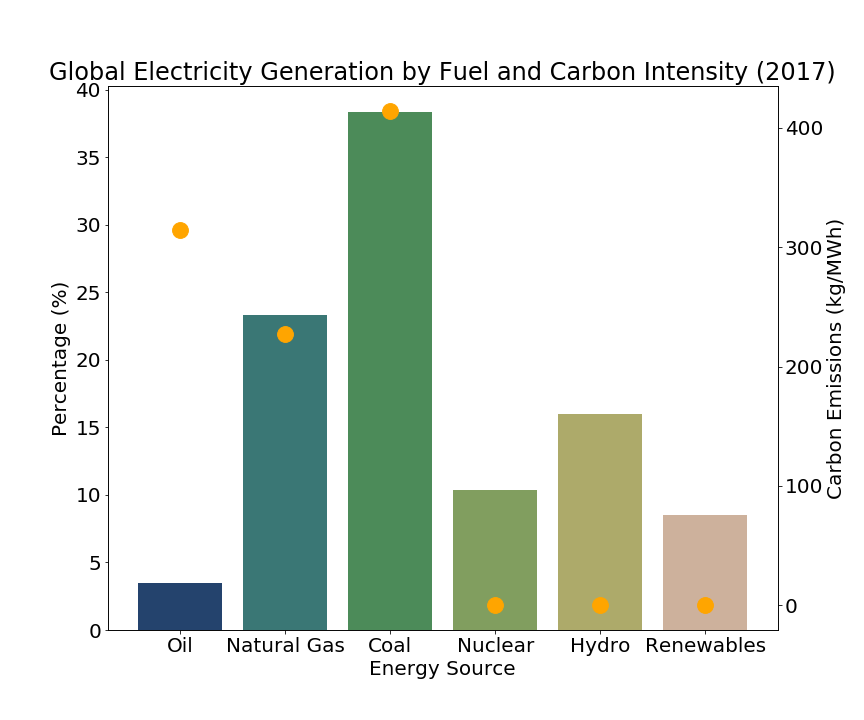
\includegraphics[width=0.45\textwidth]{figures/elec_gen_carbon.png}
		\caption{Global electricity generation sources and relative carbon emission intensity. ~\cite{BP2018,Hall1983}}
		\label{fig:fuel_emissions_market_share}
	\end{center}
\end{figure}


For a low carbon energy infrastructure, a transition in the electricity mix is required. Moving from a centralised and homogenous fossil fuel-based system to a distributed system based on renewable energy and batteries. However, such a transition needs to be performed in a safe and non-disruptive manner -- it may be possible to close down all fossil fuel plants in the next year, though if this leads to electricity shortages and power cuts then this is likely to cause significant problems both for companies and homes. Therefore a stepped approach which allows seamless transfer is desirable. This may seem a simple process to achieve -- slowly phase out existing fossil fuel generators and replace by renewable sources -- however, there are many risks and uncertainties in this process. Existing power plants have an expected lifetime and their owners wish to maximise this and the profits which can be made from them, renewable sources are still developing meaning that their efficiency and reliability will change in years to come, along with the fact that most renewable sources are effected by conditions outside the control of the owners (e.g. time of day, wind speed and cloud cover) thus leading to a need for electricity storage. 

To better understand the risks and uncertainties surrounding this transition, and to model the potential actions that can be taken by policy makers, this paper presents ElecSIM, an open source agent-based modelling toolkit, written in Python, which allows for the evaluation of alternative scenarios prior to implementation of policy. Through simulation we can evaluate many strategies in order to identify those most likely to achieve our requirements of rapid but non-disruptive migration from fossil to renewable.

This tool can be used by:
\begin{itemize}
	\item {\bf Policy experts} to test policy outcomes under different scenarios and provide quantitative advice to policy makers. They can provide a simple script defining the policies they wish to use along with the parameters for these polices.
	\item {\bf Energy market developers} who can use the extensible framework to add such things as new energy sources, policy types, consumer profiles and storage types. Thus allowing ElecSIM to adapt to a changing ecosystem.
\end{itemize}
International agreements such as the Paris climate agreement \cite{May2002}, where nation states agreed on the goal of limiting the rise in global average temperature to well below 2$^\circ$C above pre-industrial levels, mean that an open-source, reproducible and transparent model that can be utilised by experts and understood by non-experts is of importance. This allows for the development of policies based on known assumptions, thorough testing and validation.

Mathematical optimisation is often used to determine the least-cost energy infrastructure to attain specified goals \cite{Papadelis2012}. For example, calculating the optimum mix of power plant types to attain the cheapest electricity supply. Optimisation models, therefore, provide information for governments to make investment decisions in power generators over a long-term time scale. 

However, in many Western democracies, the government has liberalised energy markets, with control given to heterogeneous, private investor companies. Agent-based modelling offers a way to model these heterogeneous investor agents, and observe changes in investment decisions based on policies such as carbon tax or subsidies.

Due to the long construction times, long operating periods and high costs of power plants, investment decisions can impact electricity supply over a long time scale \cite{Chappin2017}. Governments, and society, therefore have a role in ensuring that the negative externalities of pollution and carbon emission are priced into electricity generation so that optimal decisions are made. Due to the absence of central control in electricity generation investment, other methods must be used to influence the independent players of the electricity market. Methods such as carbon taxes, policy and regulation can aid in the goals of reducing carbon emissions to limit global warming, as agreed in the Paris agreement \cite{May2002}.

 {\color{red} A diagram showing the different players, who can influence them and how?}

This paper details our model, ElecSIM. Section \ref{Literature Review} is a literature review of the models currently used in practice. Section \ref{Model} details the model and assumptions made, and section \ref{Valdiation and Performance} details how we validated our model, and displays performance metrics. Section \ref{Scenario Testing} details our results, and explores ways in which ElecSIM can be used. We conclude the work and propose future work in section \ref{Conclusion}



%\begin{itemize}
%	\item We have developed a framework for evaluating alternative scenarios, prior to implementation of policy.
%	\item Used by experts working in collaboration with policy makers.
%	\item Importance of a transition in electricity infrastructure (Paris agreement, UK Climate change act)
%	\item Importance of understanding effect of decisions made today on the future (limit of 1.5C by 2050)
%	\item Introduce ElecSIM as a toolkit to inform long-term domestic policy questions in the electricity market. 
%	\item Ability to model the effects of carbon taxation, and the effect of different scenarios 
%	\item Talk about the need to model a non-stationary, dynamic system, with multiple interacting agents with imperfect information
%	\item Requirement for an Open-Source, free Toolkit written in python. Low barrier of entry, and integration with existing python data analytics and machine learning techniques. Transparent, reproducible, and data made available. This allows for results to be open to greater criticism and better inform policy decisions.
%	\item Simple model which matches real life behaviour for low complexity and therefore increases transparency.
%\end{itemize}

